\batchmode
\documentclass{beamer}
\usepackage[utf8]{inputenc}
\usepackage[ngerman]{babel}
\usepackage{amsmath}

\usetheme[deutsch]{KIT}
\author{Jan Haag (jan.haag@student.kit.edu)}
\title{Programmieren Tutorium 10 -- Fehler und Testen}
\institute{Institut f\"{u}r Zeritfizierbare und Vertrauensw\"{u}rdige Informatiksysteme (ZVI)}
\TitleImage[scale=0.225]{frontpic.jpg}

\begin{document}
\begin{frame}
\maketitle
\end{frame}

\begin{frame}
\frametitle{Inhalt}
\tableofcontents
\end{frame}

\section{Fehler}
\begin{frame}[fragile]
\frametitle{Fehler}
\begin{verbatim}
double d = 3.14 / Integer.parseInt("Hallo...");
\end{verbatim}
\pause
L\"{o}sung: Exceptions
\end{frame}

\begin{frame}[fragile]
\frametitle{Fehler}
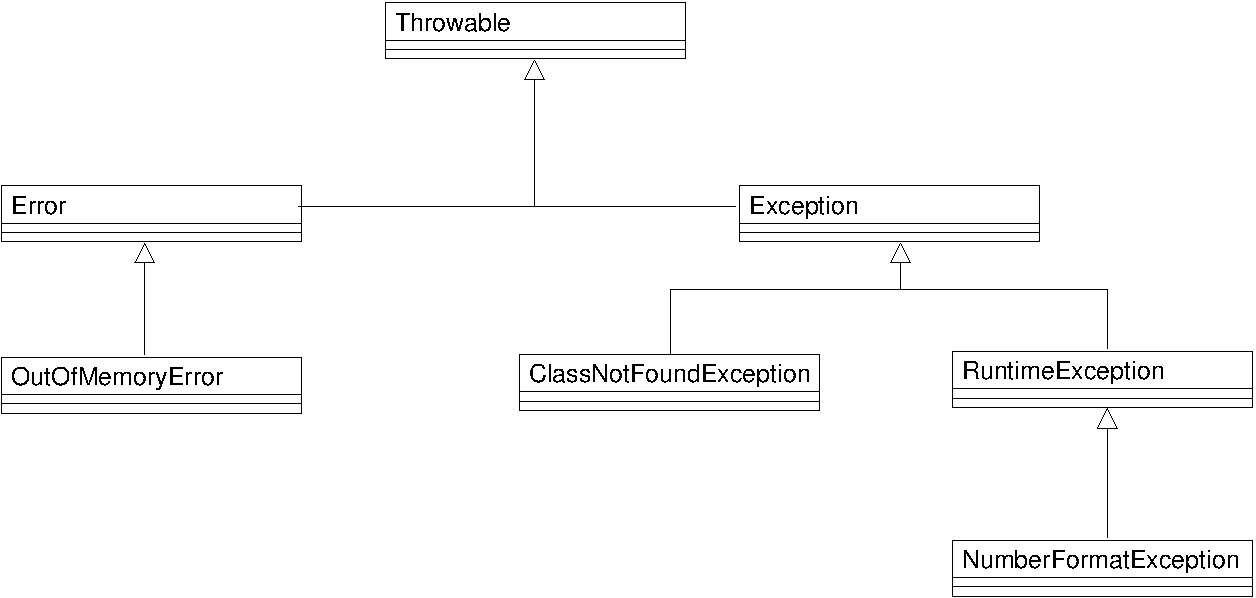
\includegraphics[scale=0.5]{ThrowableClasses.pdf}
\end{frame}

\section{Testen}
\begin{frame}
\frametitle{Testen}
I. A. Nicht ersch\"{o}pfend m\"{o}glich.
\pause
\begin{itemize}
\item Randf\"{a}lle
\item Vorherige Fehler (Regressionstest)
\item Bekannt problematische Zweige (i. e. if-then-else)
\end{itemize}
\end{frame}

\subsection{Assertions}
\begin{frame}[fragile]
\frametitle{Assertions -- Mini-Tests}
Syntax:\\
\verb|assert Logischer Ausdruck;|
\verb|assert Logischer Ausdruck: "Erklaerung";|\\
\pause
Assertions m\"{u}ssen explizit eingeschaltet werden (via \verb|-ea| parameter der JVM)
\end{frame}

\section{Aufgaben}
\begin{frame}
\frametitle{Aufgabe}
Finde und schreibe sinnvolle Tests zu \"{U}bungsblatt 4
\end{frame}

\begin{frame}
\frametitle{Ende}
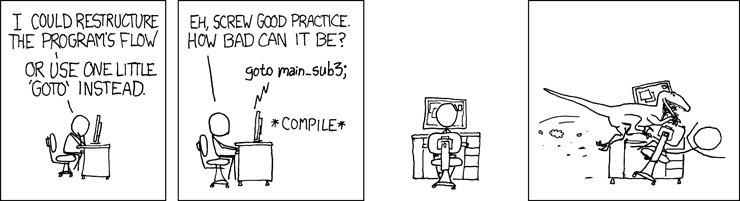
\includegraphics[scale=5.0]{goto.png}
\end{frame}
\end{document}
